% =====================================================================
% Exact Top-K Selection on a Dataflow Many-Core:
% A Measured Design-Space Study
%
% Target: IPDPS 2027 — 10 pages double-column IEEEtran (conference),
% references unlimited, DOUBLE-ANONYMOUS submission.
%
% ANONYMITY RULES (enforced in every section file):
%   - no author names, affiliations, or acknowledgments
%   - no repository URLs, no branch names, no commit hashes
%   - no "our prior paper" self-citations in the first person
%   - naming the hardware (Tenstorrent Blackhole p150a) is fine
%
% EVIDENCE RULE: every number in this paper traces to
%   paper-topk/evidence/paper/evidence.md (claim -> artifact map).
%   Numbers not in the evidence pack are forbidden; write
%   [MISSING-EVIDENCE: what] instead. See briefs/ for per-section
%   claim ownership.
%
% CLOCK CAVEAT (mandatory, methodology + every derived-us caption):
%   cycle -> microsecond conversions assume a 1.35 GHz busy clock;
%   the clock under load has not been captured (idle 800 MHz measured).
% =====================================================================
\documentclass[conference]{IEEEtran}
\IEEEoverridecommandlockouts

\usepackage{amsmath,amssymb}
\usepackage{graphicx}
\usepackage{booktabs}
\usepackage{multirow}
\usepackage{xspace}
\usepackage[caption=false,font=footnotesize]{subfig}
\usepackage{xcolor}
\usepackage{balance}
% hyperref last; hidelinks keeps the anonymous PDF clean
\usepackage[hidelinks]{hyperref}

\graphicspath{{fig/}}

% ---- shorthand macros (keep numbers consistent across sections) ----
\newcommand{\topkop}{\texttt{topk\_large\_indices}\xspace}
\newcommand{\ttnntopk}{\texttt{ttnn.topk}\xspace}
\newcommand{\bh}{Blackhole\xspace}
\newcommand{\pca}{p150a\xspace}
\newcommand{\us}{\,\textmu s\xspace}
% cost model, typeset once, reused everywhere
\newcommand{\costmodel}{$2\lceil C/P\rceil + \lceil \log_2 P\rceil$\xspace}
% draft-only marker for numbers awaiting evidence (must be empty at submission)
\newcommand{\missing}[1]{\textcolor{red}{[MISSING-EVIDENCE: #1]}}

\begin{document}

\title{Exact Top-K Selection on a Dataflow Many-Core:\\
A Measured Design-Space Study}

% ---- DOUBLE-ANONYMOUS: do not edit ----
\author{\IEEEauthorblockN{Anonymous Authors}
\IEEEauthorblockA{Paper \#XXX --- IPDPS 2027 submission}}

\maketitle

% Abstract + keywords live with the introduction brief (briefs/01-intro.md)
% Abstract — owned by briefs/01-intro.md.
% Every number traces to paper-topk/evidence/paper/evidence.md:
%   H1 (9,956x), H2 (34.3us@32c, 18,401x), H3 (23.3us@104c), H4 (9.7-29.9x),
%   C1-1/C1-3/C1-5 (counting/decision/materialization), C2-1 (cost model),
%   C3-1/C3-4 (skip law, 1.82x), C4-1..C4-3 (characterization), C1-6 (honest frame).
% All microsecond values here are Tracy-measured at op level (no cycle
% conversion), so the 1.35 GHz caveat does not attach; cycle figures stay in cycles.
\begin{abstract}
Exact top-$k$ selection sits on the decode-time critical path of large
language model serving: sampling selects $k{=}32$--$64$ winners from a padded
vocabulary shard every token, sparse-attention indexers select
$k{=}512$--$2048$ keys per layer, and mixture-of-experts gates fire every
forward pass. GPU practice treats the problem as solved---count, partition,
scatter, repeat---while accelerator studies either approximate the selection
or never measure it. We present a measured design-space study of exact
top-$k$ on a Tenstorrent Blackhole \pca, a dataflow many-core with 130 Tensix
workers on a 13$\times$10 mesh NoC, software-managed SRAM, and neither
atomics nor scatter in the compute path. Single-ingredient silicon
microbenchmarks show why GPU radix-select economics do not transfer: exact
SFPU counting yields 1 bit per 2.0 cycles/vector, a count-to-decision
rendezvous costs 81 cycles, and materialization---not counting---is the load-bearing gap
(dense emission 13.0 cycles/element against a 0.5 bar). The design space
instead rewards parallelizing the data-oblivious comparison network: a
column-parallel log-tree operator whose bitonic leaves feed a semaphore-tree
merge, governed by a validated cost model \costmodel. The operator measures
34.3\us at $k{=}2048$, $N{=}65{,}536$ (bf16) on 32 cores---18,401$\times$
over the pre-study stock path---and scales monotonically to 23.3\us at
$k{=}512$, $N{=}262{,}144$ on 104 cores. A distribution-free chunk-skip law
$P(\mathrm{skip}) \approx e^{-K/(c+1)}$ with a compile-time $K/4$ gate adds
1.82$\times$ ($-45.1\%$) at $k{=}32$, $N{=}65{,}536$. End to end, the
user-facing \ttnntopk call at $k{=}2048$, $N{=}65{,}536$ improves from
631.5\,ms to 63.4\us---9,956$\times$---and the surviving gap to the vendor
roofline spans 9.7--29.9$\times$ across all 24 measured cells. The study is
honest about its own dynamics: the incumbent bitonic engine absorbed the
study's routing and placement fixes and outran the radix-select model it was
measured against. We also report the first public characterization of the
Tensix datapath's numeric semantics: bf16 canonicalization, a native
sign-magnitude total order including NaN, and a 1-in-8-sampled, 32-bin-aliased
packer exponent histogram.
\end{abstract}

\begin{IEEEkeywords}
top-k selection, dataflow architectures, network-on-chip, many-core,
Tenstorrent Blackhole, performance characterization
\end{IEEEkeywords}


% Introduction — owned by briefs/01-intro.md.
% Evidence trace: hook = scenarios1_table.csv row sampling_qwen36_tp4 (9,596.29 us,
% k=32, N=65,536, 1 core) + H6 (~137 ns/elem linear factory); thesis = H1
% (631.5 ms -> 63.4 us, 9,956x, prebranch->routed chain); contributions C1-C4
% carry their evidence.md anchors. Chains never mixed: 9,956x is
% prebranch->routed (ttnn.topk); 18,401x is prebranch->op. No roofline-v2
% claim (G6 unresolved); blaze absent; no repo URLs/hashes (double-anonymous).
% All us values Tracy-measured (no 1.35 GHz caveat needed); cycles stay cycles.
\section{Introduction}
\label{sec:intro}

On a
Tenstorrent \bh \pca, Qwen3 decode sampling under tensor parallelism~4 shards
a 151{,}936-entry vocabulary into 37{,}984 logits per device and pads the
shard to 65{,}536---the one power-of-two width that fails the shipping
bitonic engine's $W{<}65{,}535$ routing gate. The call lands on a single-core
linear factory that walks logits at ${\approx}137$\,ns/element: 9{,}596\us
per sampled token for a $k{=}32$ selection, while the other 129 cores idle.
The cliff is not a corner case. At the sparse-attention indexer shape
$k{=}2048$, $N{=}65{,}536$ (bf16), the stock \ttnntopk path measured
631.5\,ms per call at the start of this study; the same call on the same
silicon now measures 63.4\us---9{,}956$\times$---with no new hardware. This
paper argues one sentence: exact top-$k$ on a commercial NoC-mesh dataflow
chip sat four orders of magnitude off its achievable floor, and a measured
design-space study---not a clever new algorithm---closed the gap.

\bh is a dataflow many-core: 130 Tensix workers on a 13$\times$10 grid, each
with five RISC-V processors, a 32-lane SIMD unit (SFPU), and software-managed
SRAM, joined by a 2D NoC~\cite{vasiljevic2024blackhole}. Every fast GPU
top-$k$ mechanism leans on primitives this machine lacks --- atomic
histograms, scatter compaction, grid-wide
synchronization~\cite{alabi2012kselection,gaihre2021drtopk,li2024radik}
(\S\ref{sec:bg-problem}).

The missing primitives are not one vendor's oversight. AI accelerators
across the industry traded coherent shared memory and atomics for mesh
bandwidth and software-managed SRAM, because matrix multiplication rewards
the trade. Selection is the canonical data-dependent workload the trade
punishes, and LLM decoding keeps placing it on the critical path
(\S\ref{sec:bg-problem} fixes the data
contract)~\cite{fan2018topk,deepseekv32,gvr2026,shazeer2017moe}. Nobody
has measured what the trade costs here: no sorting or selection
publication exists for the dataflow-accelerator class
(\S\ref{sec:related}), and TPU studies escape into
approximation~\cite{chern2022tpuknn,twostage2025}. Mesh-selection theory
proved step bounds on abstract
arrays~\cite{krizanc1992optimal,krizanc1993fast}, but returned neither
values-with-indices nor silicon measurements.

We measured the design space ingredient by ingredient instead of betting on
one kernel. The study decomposes every exact top-$k$ engine along three
questions---winner identification, data touched per pass, decision cost
between passes---and holds \bh against each with
single-ingredient microbenchmarks (\S\ref{sec:design-space}). The answers
overturn the GPU playbook: counting is narrow, decisions are affordable, and
materialization is the wall, so radix select degenerates to threshold
bisection and loses. The space instead rewards parallelizing the
data-oblivious comparison network as a column-parallel log-tree operator
(\S\ref{sec:system}); the one data-dependent mechanism that survives without
scatter is a chunk-skip rule, sound by construction and gated at
compile time by a distribution-free rank-statistic law.

The study is candid about its own dynamics. The incumbent bitonic engine
absorbed the study's routing and placement fixes and finished at 34.4\us on
the anchor cell ($k{=}2048$, $N{=}65{,}536$)---inside the uncertainty band
of the radix-select model priced from our own microbenchmarks; a
pre-registered stop rule closed that track (\S\ref{sec:design-space}).
The same candor governs the headline: \S\ref{sec:eval-attribution}
attributes the orders of magnitude mostly to routing around the
single-core fallback, and the algorithm to a measured 1.4$\times$ over
the strongest eligible stock configuration plus its measured tree,
placement, and skip terms. The surviving gap to the
vendor roofline is 9.7--29.9$\times$ across all 24 measured cells
(\S\ref{sec:evaluation}).

This paper contributes:
\begin{itemize}
\item \textbf{Quantification}, via single-ingredient silicon
  microbenchmarks, of why GPU radix-select economics do not transfer to
  a NoC-mesh dataflow core: counting is narrow, decisions are
  affordable, and materialization---not counting---is the load-bearing
  gap (\S\ref{sec:design-space}).
\item \textbf{Design and measurement} of a column-parallel log-tree top-$k$
  operator---semaphore-tree rendezvous without
  atomics or global synchronization---with the validated cost model
  \costmodel and a cost-optimal rectangle embedding: 34.3\us at $k{=}2048$,
  $N{=}65{,}536$ on 32 cores (18{,}401$\times$ over the pre-study stock
  \ttnntopk) and monotone scaling to 23.3\us at $k{=}512$, $N{=}262{,}144$
  on 104 cores (\S\ref{sec:system}, \S\ref{sec:evaluation}). To our
  knowledge, the first \emph{measured} full top-$k$ (values and indices) on
  commercial NoC-mesh silicon (\S\ref{sec:related}).
\item \textbf{Derivation and silicon validation} of a distribution-free
  chunk-skip law $P(\mathrm{skip}) \approx e^{-K/(c+1)}$
  for streaming bitonic cascades, with a soundness proof, a compile-time
  $K/4$ gate, and a calibrated pre-build forecast that eliminated the losing
  variant; the surviving variant measures 1.82$\times$ at
  rows${=}2$, $k{=}32$, $N{=}65{,}536$ (\S\ref{sec:system}).
\item \textbf{First public characterization} of the Tensix compute
  datapath's numeric semantics and sorting-relevant primitive costs: bf16
  canonicalization (NaN$\to$Inf, $-0\to{+}0$, subnormal$\to{+}0$), a native
  sign-magnitude total order including NaN, a 1-in-8-sampled and
  32-bin-aliased packer exponent histogram, and measured synchronization
  floors (\S\ref{sec:characterization}).
\end{itemize}

Every performance cell behind these claims is gated bit-exact against a host
golden and every headline number traces to
a committed measurement artifact; the ledger and canonical harness
will be released, and \S\ref{sec:methodology} discloses the agentic
campaign methodology.

% =====================================================================
% Background -- owned by briefs/02-background.md.
% Budget: 2.0 columns incl. Fig B1 (fig/fig-b1-tensix-mesh.pdf,
% generated by fig/make_fig_b1.py -- architecture drawing, no data CSV).
%
% Evidence trace (every number):
%   130 workers / 13x10 grid / p150a ... evidence.md header; Hot Chips cite
%   ~1.5 MB L1 ......................... vasiljevic2024blackhole (cited)
%   M snap rule (512/1024/2048) ........ evidence/tileskip/forecast.md S1
%   multi-core gate (pow2, W<65535,
%     k<=64, N>=4096) .................. RADIX_BUCKET_GPU.md S7.3 item 2
%   ~137 ns/elem; 695 us @ W=5000 (k32);
%     17.95 ms @ W=65536 (k64) ......... H6: baselines/smallk_routefix/
%                                        stock_nonpow2.csv + scope51 CSV
%   ~89x cliff; 106.7 us @ N=8192 (65c)
%     vs 9.49 ms @ N=65534 (1c) ........ H8: baselines/scope51/
%                                        canonical_sweep.csv
%   ~2 cyc/elem data-oblivious ......... RADIX_BUCKET_GPU.md S7.1-7.2
%   bf16 at all 8 call sites ........... baselines/comp3/scenarios1_table.csv
%   fp32 bit-exact ..................... C4-1 (stated, defended in Sec. 5)
% 2.1 Problem statement (added rev 1):
%   contract (canonicalized-input top-k multiset, sign-magnitude order,
%     x[index]==value bit-exact, bit-identical relaunches, stable=false
%     ties, valid-length prefix) ....... test_topk_contract.py docstring
%                                        (T1 tiers, I13 determinism) + M4
%   62-cell suite count ................ evidence M4 / Sec. 6-A
%   consumer classes k=32 vocab 16-65K /
%     k=512-2048 to 1M / k=4-16 over
%     128-512 experts .................. scenarios1_table.csv + callsites.md
%   81-cycle rendezvous ................ C1-3 (Sec. 3 owns the measurement)
%   CPU contrast cites (UNVERIFIED) .... blacher2023vqsort, intel_x86simdsort
%
% Cross-section \ref labels assumed (coordinate with section owners):
%   sec:design-space (S3), sec:system (S4), sec:characterization (S5),
%   sec:evaluation (S6).
% Extra bib entries: refs-extra-02-background.bib (ttnn_topk_docs,
%   ttmetal_topk_issue33492) -- merge into the bibliography at assembly.
% =====================================================================
\section{Background}
\label{sec:background}

\subsection{Problem Statement and Data Contract}
\label{sec:bg-problem}

% Contract facts: test_topk_contract.py docstring (T1 tiers, I13 determinism,
% canonicalization, sign-magnitude order); 62-cell count = evidence M4.
% Consumer shapes: baselines/comp3/scenarios1_table.csv + scenarios/callsites.md.
The object of study is exact top-$k$ selection: given one or more rows
$x \in \mathrm{bf16}^{N}$ resident in device DRAM, return the $k$ largest
elements of each row --- values \emph{and original indices}, exact rather
than approximate, sorted descending. Under \texttt{stable=false}, ties may
resolve to any valid winner set but must be deterministic for a fixed
input. A 62-cell differential contract suite pins what the shipping
engines actually promise: the returned values are the exact top-$k$
multiset of the input \emph{as canonicalized by the datapath} (bf16
specials are rewritten on entry; Section~\ref{sec:characterization} pins
the rules) under the hardware's native sign-magnitude total order; every
index is unique and satisfies $x[\mathrm{index}] = \mathrm{value}$
bit-exactly (short rows emit a documented sentinel index); repeated
launches return bit-identical outputs. bf16 is
the datatype at every surveyed production call site; fp32 traverses
bit-exactly. Production adds three contract variants:
indices-only versus (values, indices) outputs, multi-row batches, and a
valid-length prefix that masks a stale tail.

Where does $x$ come from, and where do the results go? The row is
always the upstream operator's output --- an lm-head matmul, an
attention-indexer score, or an expert-gate projection ---
DRAM-interleaved in the producer's layout; results return to DRAM. Three
consumer classes cover every surveyed call site
(Table~\ref{tab:scenarios}): token sampling needs values and indices at
$k{=}32$ over vocabulary shards of $N{=}16$--$65$K every decoded token;
sparse-attention KV gather needs indices only at $k{=}512$--$2048$ over
contexts up to 1M, every layer; mixture-of-experts dispatch needs
$k{=}4$--$16$ winners over 128--512 experts every layer. A selection engine's real cost therefore includes the layout
conversions between producer, engine, and consumer formats --- why
Section~\ref{sec:evaluation} prices end-to-end composites, never bare
kernels.

The machine class sets the difficulty. CPU selection --- vectorized
quickselect of the \texttt{x86-simd-sort}/vqsort
family~\cite{intel_x86simdsort,blacher2023vqsort} --- rides coherent
caches and branch predictors: branchy, data-dependent control flow is
cheap and the scalar pivot logic is free. GPU selection rides
shared-memory atomic histograms, scatter compaction, and grid-wide
synchronization --- Section~\ref{sec:design-space} prices each of these
affordances on this silicon. \bh has none of them: no
cross-core atomics, no scatter or compaction in the compute path, no
global barrier --- synchronization is NoC semaphores over
software-managed SRAM, the 32-lane SFPU counts 1--3 bits per pass, and
the fast path is a fixed, data-oblivious instruction stream, so every
data-dependent decision costs a measured 81-cycle rendezvous.

\subsection{Blackhole and the Tensix Core}
\label{sec:bg-tensix}

The Tenstorrent \bh \pca exposes 130 programmable Tensix workers on a
13$\times$10 grid, joined by a 2D network-on-chip
(NoC)~\cite{vasiljevic2024blackhole}; the count is a property of
this unit (harvesting varies; no result hardcodes it). Each
core owns
${\approx}1.5$\,MB of software-managed L1 SRAM~\cite{vasiljevic2024blackhole};
there is no cache hierarchy and no coherence protocol.

Five RISC-V processors share that L1: two move data over the NoC, and
three compute as an
\emph{unpack}$\to$\emph{math}$\to$\emph{pack} pipeline. The math stage
owns the SFPU, a 32-lane SIMD engine, and
stages its output in the Dst register file that pack consumes. An operator is therefore
three-to-five cooperating programs per core, synchronized through
circular buffers in L1.
Sections~\ref{sec:design-space} and~\ref{sec:characterization} price these
units one at a time; Section~\ref{sec:system} spends them.

\subsection{The Incumbent Bitonic Engines}
\label{sec:bg-incumbent}

The vendor stack routes \ttnntopk through a bitonic local sort in the
low-level kernel library
(\texttt{topk\_local\_sort})~\cite{ttnn_topk_docs,ttmetal_topk_issue33492}.
The bitonic leaf sorts a window of $M$ elements resident in Dst, where $M$
snaps upward from the requested $k$: $k\le512$ gives $M{=}512$, $k\le1024$
gives $1024$, and larger $k$ gives $2048$. We fix the paper's notation here:
a row holds $N$ elements, split into $C = N/M$ chunks; $P$ cores cooperate on
one row; $K$ is the user's $k$. All later sections inherit these symbols.

Before this study, two engines shipped. A multi-core bitonic path accepts
only rows with power-of-two width, $W < 65{,}535$, $k \le 64$, and
$N \ge 4096$. A single-core linear factory catches everything else at
${\approx}137$\,ns/element: 695\us at $W{=}5{,}000$ ($k{=}32$), growing to
17.95\,ms at $W{=}65{,}536$ ($k{=}64$). Between the two engines sits a
measured cliff. At the $W < 65{,}535$ gate, a $k\le32$ row jumps from
106.7\us (multi-core, 65 cores, $N{=}8{,}192$) to 9.49\,ms (one core,
$N{=}65{,}534$) --- ${\approx}89\times$ more time for $8\times$ more
elements. The cliff is architecture context here;
Section~\ref{sec:evaluation} owns the fix. The bitonic engine itself is
data-oblivious --- one corner of the design space
Section~\ref{sec:design-space} maps and prices.

Exact GPU top-k, by contrast, is a mature family, each branch leaning
on a hardware affordance \bh must re-price to import: radix/bucket
select on 8--12-bit atomic histograms plus scatter
compaction~\cite{alabi2012kselection,zhang2023paralleltopk,li2024radik};
WarpSelect on a cheap per-lane running-threshold compare with per-lane
survivor queues~\cite{johnson2019billion}; threshold-guess decoders on
cheap counting against a predicted boundary~\cite{gvr2026}; and
TPU-KNN's escape into matmul-shaped
approximation~\cite{chern2022tpuknn,twostage2025}. This paper measures
the exact path anyway: Section~\ref{sec:design-space} prices each
affordance on silicon.

% Why GPU Selection Economics Do Not Transfer -- owned by briefs/03-design-space.md.
% Every number traces to paper-topk/evidence/paper/evidence.md rows C1-1..C1-7
% (sources: cgtceq-debug.md, risc_scan_bench, RADIX_BUCKET_GPU.md section 7).
% Figures: fig/fig-d1-design-space.pdf, fig/fig-d2-engine-shootout.pdf
% (generated by fig/make_figs_03.py). Extra bib: refs-extra-03-design-space.bib
% (floydrivest1975, shared key with section 07's extra bib) -- merge at integration.
\section{Why GPU Selection Economics Do Not Transfer}
\label{sec:design-space}

GPU radix select wins because its hardware sells wide exact counting and
cheap
materialization~\cite{alabi2012kselection,gaihre2021drtopk,zhang2023paralleltopk,li2024radik};
\bh quotes different prices. This section decomposes exact selection into
three orthogonal questions, prices each ingredient on silicon, and locates
the ingredient that kills the family --- materialization, not counting and
not synchronization. The (A)--(F) vocabulary defined here carries through
Sections~\ref{sec:system}--\ref{sec:conclusion}.

\subsection{Three Questions, Six Answers}
\label{sec:dspace-map}

Every exact top-k engine answers three independent questions.
\textbf{Q1 --- winner identification:} either \textbf{(A)}~a comparison
network --- a fixed, data-oblivious schedule of compare--exchanges
(bitonic sort/merge, WarpSelect~\cite{johnson2019billion}) --- or
\textbf{(B)}~counting/partitioning, which counts elements beyond a
boundary and \emph{decides} where to look next.
\textbf{Q2 --- data touched per pass:} either \textbf{(C)}~full-data
passes every time, or \textbf{(D)}~shrinking candidate sets, by scatter
compaction or count-guided skipping.
\textbf{Q3 --- decision cost between passes:} \textbf{(E)}~nothing, for
oblivious schedules; or \textbf{(F)}~a synchronization rendezvous that
carries the count to a scalar decision-maker and redistributes the
verdict.

GPU radix select answers (B)+(D)+cheap-(F): 8--12-bit atomic histograms,
scatter compaction, grid-sync decisions
(Section~\ref{sec:background})~\cite{alabi2012kselection,li2024radik};
the shipping \bh engine answers (A)+(C)+(E) --- $\approx$2 cycles/element
on every pass, zero decisions. Can \bh move to (B)?

\begin{table}[t]
\caption{GPU radix-select ingredients, priced on \bh.}
\label{tab:ingredients}
\centering
\scriptsize
\setlength{\tabcolsep}{3pt}
\begin{tabular}{@{}p{1.3cm}p{1.1cm}p{3.9cm}p{1.5cm}@{}}
\toprule
\textbf{Ingredient} & \textbf{GPU form} & \textbf{\bh, measured} & \textbf{Verdict} \\
\midrule
Wide exact counting (Q1-B) &
8--12 bits/pass, shared-mem.\ atomics~\cite{alabi2012kselection,li2024radik} &
SFPU: 1\,bit @ 2.0 cyc/vec, 3\,bits @ 3.0; additive on the 3.94 cyc/vec
unpack floor ($+$2.42/$+$4.52 in-stream; 2.44/4.53 isolated)
[\texttt{cgtceq}]. RISC: 256-bin histogram
7.56--7.90 cyc/elem vs.\ 3.02 load floor; 8.23 with 4-way sub-histograms;
L1-resident 15.5--19.9 [\texttt{risc-scan}] &
narrow (SFPU) or slow (RISC) --- degenerates to bisection \\
\addlinespace
Cheap decisions (Q3-F) &
grid sync / fused kernels &
81 cyc/decision best (sync $+$ fold $+$ MMIO read); semaphore 101, sentinel
98; no fold 756--773; MMIO $\approx$10 cyc/word [\texttt{cgtceq}] &
affordable --- not the blocker \\
\addlinespace
\hspace{0pt}Materiali\-zation (Q2-D) &
scatter / compaction &
dense RISC emit 12.97--17.81 cyc/elem vs.\ a $\approx$0.5 bar; SFPU has no
scatter; packer compressed stream 0.63 cyc/orig-elem, consumer-only
[\texttt{risc-scan}] &
the load-bearing gap \\
\addlinespace
A slow incumbent &
\texttt{thrust::} \texttt{sort} &
34.4\us (k=2048, N=65{,}536); 23.3\us (k=512, N=262{,}144) after this
study's own fixes [\texttt{sweep}] &
bar moved $-$15--27\% during the study \\
\bottomrule
\end{tabular}
\end{table}

\subsection{The Ingredients, Measured}
\label{sec:dspace-ingredients}

Table~\ref{tab:ingredients} prices the four ingredients, each cell tagged
with its benchmark; all costs are slope-measured cycles,
gated bit-exactly against host goldens (\S\ref{sec:eval-method}).

\textbf{Wide exact counting (Q1-B).}
The 32-lane SFPU counts exactly but narrowly: one predicate bit per pass
at 2.0000 cycles/vector, three bits at 3.0, riding additively on the 3.94
cyc/vec unpack floor. A GPU pass
resolves 8--12 bits~\cite{alabi2012kselection,li2024radik}; an SFPU pass
resolves 1--3, so a radix engine on this datapath collapses into a
bisection. The scalar cores are no rescue: a 256-bin RISC histogram runs
7.56--7.90 cycles/element against a 3.02 pure-load floor.

\textbf{Cheap decisions (Q3-F).}
Decisions measure 81 cycles each at best: a \texttt{tensix\_sync}, a
cross-lane SFPU fold, and one memory-mapped read of the \textsc{Dst}
register file (folding is mandatory --- raw-lane reads cost 756--773
cycles, $\approx$9$\times$ worse). At 81 cycles $\approx$ 60\,ns\footnote{%
Cycle$\to$time conversions assume a 1.35\,GHz busy clock; the clock under
load has not been captured (idle 800\,MHz measured).
Section~\ref{sec:evaluation} states the caveat once for the whole paper.}
and $\approx$14 decisions per row
(Section~\ref{sec:dspace-bisection}), decisions are affordable --- not
the blocker.

\textbf{Materialization (Q2-D).}
Dense survivor emission on a RISC core measures 12.97--17.81
cycles/element against a $\approx$0.5 cycles/element bar for compaction to
pay --- dead. The SFPU has no scatter path at all. The sole survivor, the
packer's zero-compressed output stream with a skip-zero RISC consumer,
costs 0.63 cycles per original element: $\approx$3$\times$ under one
bitonic leaf pass but 2--5$\times$ above GPU-paper compaction --- and it
is consumer-only, measured on uniform input: no device-side decoder
exists, and the composed producer$+$consumer cost was never measured ---
reopening condition~\#1 in Section~\ref{sec:conclusion}.

\subsection{Degeneration to Threshold Bisection}
\label{sec:dspace-bisection}

Without (D), every counting pass is strictly additive to the bitonic
finish that must still run; what survives of (B) is threshold bisection
on the key space, monotone because sign-magnitude keys order the probes
(Section~\ref{sec:characterization}). Over 57 input cells ---
random, clustered, and all-equal distributions across seeds, a
$K\in\{31,32,33\}$ straddle, ties, and $\pm 0$/Inf/NaN/denormal specials
--- bisection to the exact $K$-th threshold costs a median of 14 decisions
and 2{,}313 cycles per 1{,}024-element row, worst case 17
decisions on clustered, all-equal, and tied inputs, exactly where
key-space bisection predicts; the certification invariant
$C_{\mathrm{gt}} < K \le C_{\mathrm{gt}}{+}C_{\mathrm{eq}}$ held
field-exactly on every row. Per decision, $\approx$165 cycles --- one
count pass ($\approx$64--70), one rendezvous (81), loop
overhead: the (F) matrix composes as priced. At $\approx$1.7\us per row
the exact arm is honest ---
Floyd--Rivest economics~\cite{floydrivest1975}, not radix
economics. The family fits \bh only in its degenerate corner, (B)+(C)+(F).

\subsection{Why the Track Closed}
\label{sec:dspace-closure}

A selector composed from the measured components --- packer pre-filter,
count passes, rendezvous, materialization, final $K$-sort --- prices at
$\approx$21--30\us per large cell. The pre-registered stop rule, written
before any measurement, demanded an incumbent $\ge$2$\times$ the model to
justify building. The incumbent finished the study at 34.4\us (k=2048,
N=65{,}536) --- inside the model's uncertainty band --- because the
study's own first gate produced two structural fixes (a small-k routing
repair and a core-count cap raise, Sections~\ref{sec:system}
and~\ref{sec:evaluation}) that made the incumbent 15--27\% faster while
the selector was being priced. A selector that must outrun its own
evaluation's side effects is not a production bet; the track closed by
its own rule. The machinery was banked: the rendezvous and fold
primitives price Section~\ref{sec:system}'s chunk-skip decision; the
floors join Section~\ref{sec:characterization}.

% A Log-Tree Top-K Engine for a NoC Mesh -- owned by briefs/04-system.md.
% Evidence: C2-1..C2-5, C3-1..C3-6 (evidence.md sections 1.3, 1.4), H11;
% forecast.md sections 1-5; rowskip-implementation.md sections 1-7;
% contrast rows from related-work.md section 3.
% Anonymity: kernels described structurally; no repo paths, no hashes.
\section{A Log-Tree Top-K Engine for a NoC Mesh}
\label{sec:system}

The map of Section~\ref{sec:design-space} leaves two live moves. First,
parallelize the data-oblivious corner (A)+(C)+(E): split the row across
cores and pay a log-depth rendezvous instead of a shared-memory partition.
Second, import the shrinking axis (D) in the only form that survives
without scatter: skip work, never move data. This section builds both:
Sections~\ref{sec:tree}--\ref{sec:costmodel} the column-parallel log-tree
operator (\topkop), Sections~\ref{sec:skip-mech}--\ref{sec:forecast}
chunk-skip and the calibrated forecast that eliminated its losing variant
pre-build.

\subsection{Operator Structure}
\label{sec:tree}

Figure~\ref{fig:operator} shows the operator on one row of $N$ elements,
using the notation of Section~\ref{sec:background}: the leaf window $M$
snaps to the LLK sort width (\S\ref{sec:bg-incumbent}), and the row
splits into
$C = N/M$ chunks. The program places $P$ slices on a rectangle of cores;
each slice streams $\lceil C/P \rceil$ chunks through a bitonic leaf that
sorts the arriving chunk, merges it into a resident $M$-wide descending
window, and rebuilds the window order. A $\lceil \log_2 P \rceil$-level
in-place merge tree --- the mesh-shaped sibling of FPGA merge-tree
sorters~\cite{samardzic2020bonsai}, applied to selection --- then folds
the $P$ windows to a root core, which emits the top-$K$ values and
indices; every level halves the live cores and merges two $M$-wide
sequences.

The synchronization fabric is deliberately austere. Tree levels map
one-to-one onto NoC semaphore levels; each core owns a single receive
circular buffer sized for two $M$-wide sequences; the writer kernels
extend to seven partner slots, enough for $P{=}128$. The operator uses no atomics, no
global barrier, and no dedicated DRAM scratch
(\S\ref{sec:bg-problem})~\cite{alabi2012kselection,li2024radik}. The tree
replaced a serial merge-chain ancestor that folded slices one at a time:
at fixed core counts the swap cut $k{=}2048$, $N{=}65{,}536$ from
69.6\us{} to 41.9\us{} (1.66$\times$) and $k{=}512$, $N{=}262{,}144$ from
64.2\us{} to 32.0\us{} (2.01$\times$), and it made runtime monotone in
$P$ --- the property the cost model below then exploits.

\begin{figure}[t]
  \centering
  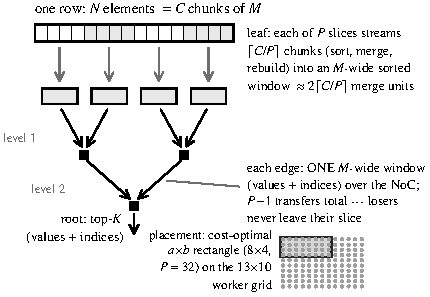
\includegraphics[width=0.75\linewidth]{fig-s1-operator.pdf}
  \caption{Column-parallel log-tree top-$k$ operator.}
  \label{fig:operator}
\end{figure}

\subsection{Cost Model and Rectangle Embedding}
\label{sec:costmodel}

The factory chooses $P$ by minimizing a two-term model in leaf merge
units:
\begin{equation}
  \mathrm{cost}(P) \;=\; 2\,\big\lceil C/P \big\rceil
  \;+\; \big\lceil \log_2 P \big\rceil,
  \qquad P \in [2,\, \min(C, 128)],
  \label{eq:costmodel}
\end{equation}
with ties resolved toward fewer cores. The factor of two prices the leaf
honestly: every chunk after the first costs $\approx$2 merge units (sort,
merge, rebuild) while chunk~0 costs one. The unit constant is measured,
not assumed: 1.46\us{} per merge unit at $M{=}512$ and 5.51\us{} at
$M{=}2048$ ($\approx$1{,}966 and $\approx$7{,}440
cycles\footnote{\label{fn:clock}Cycle forms of Tracy-measured times assume
a 1.35\,GHz busy clock; the clock under load was not captured (idle
800\,MHz measured). Section~\ref{sec:evaluation} states the policy; all
cycle$\rightarrow$time conversions in this section carry it.}). The leaf
term is mesh-selection theory's multi-packet
regime~\cite{krizanc1992optimal,krizanc1993fast,multipacket1992} with
measured constants; the log term is the mesh's rendezvous price.

Minimizing Eq.~\ref{eq:costmodel} is only half the placement problem; the
winner must also embed in the 13$\times$10 worker grid as a contiguous
$a{\times}b$ rectangle. An earlier full-rows-only fit silently clamped
$P$: at $k{=}2048$, $N{=}65{,}536$ it settled for 13$\times$2 = 26 cores
while an 8$\times$4 = 32-core rectangle sat free. Searching all
cost-optimal rectangles instead wins 8--27\% at the op level across the
re-pinned cells: 41.9$\rightarrow$34.4\us{} (26$\rightarrow$32 cores),
58.6$\rightarrow$49.6\us{} (52$\rightarrow$64), 32.0$\rightarrow$23.3\us{}
(52$\rightarrow$104), and 15.0$\rightarrow$13.1\us{}
(52$\rightarrow$64). On a harvested mesh the
embedding search is part of the cost model, not a detail below it.
Section~\ref{sec:eval-scaling} defends the model against the measured
15-point $P$-sweep, including the ceiling-term bump it predicts.

\subsection{Chunk-Skip: Mechanism and Soundness}
\label{sec:skip-mech}

Ingredient (D) --- shrinking the touched data --- survives on this
machine only if nothing has to move. Chunk-skip is that import: a
per-chunk predicate that decides whether the leaf pipeline needs to run
at all. Let $T$ be the running $K$-th largest survivor, read from the
resident sorted window. The rule is strict:
skip chunk $c$ iff $\max(\text{chunk}_c) < T$. Chunk~0 always seeds the
window; $T$ is monotone nondecreasing because merges only improve the
window; boundary ties ($\max = T$) are never skipped; and the decision is
a pure function of the input, so the output is deterministic per input.

Soundness admits a short argument: at most $K{-}1$ elements ever exceed
the row's final $K$-th largest value $v_K$, so $T \le v_K$ at all times;
any member $x$ of an exact top-$K$ set satisfies $x \ge v_K \ge T$, so
the strict test never fires on $x$'s chunk, and $x$, sitting within the
top-$K \le$ top-$M$, survives every $M$-wide merge to the root. The
released kernel source carries the full 288-line proof as a header
comment. The contrast with the GPU running-threshold family is
threefold: WarpSelect thresholds per element, with no analytic skip
law~\cite{johnson2019billion}; GVR guesses its threshold from the
previous decode step and must count, verify, and refine after a
misprediction~\cite{gvr2026}; chunk-skip prunes at $M$-element
granularity, sound by construction --- no verification pass exists to
pay for --- with a distribution-free law and compile-time gate
(\S\ref{sec:skip-law}) and a pre-build forecast (\S\ref{sec:forecast})
that neither GPU mechanism has. Adversarial validation
backs the proof: a 36-check battery (all-equal, ascending, last-chunk
winners, boundary ties replicated across 64 chunks) is bit-exact in both
gated and ungated configurations, and a 20-launch hang battery passed
twice.

\subsection{The Skip Law and Its Compile-Time Gate}
\label{sec:skip-law}

How often the rule fires is a rank statistic, not a distribution
property. For i.i.d.\ inputs, chunk $c{+}1$ is skippable iff the top-$K$
of the first $(c{+}1)M$ elements all lie in the first $cM$:
\begin{equation}
  \Pr[\text{skip at } c] \;=\;
  \binom{cM}{K} \Big/ \binom{(c+1)M}{K}
  \;\approx\; e^{-K/(c+1)},
  \label{eq:skiplaw}
\end{equation}
identical for normal, uniform, and softmax-shaped inputs because only
ranks enter. The law is unforgiving at short streams: a
conservative $K{=}512$ threshold skips with probability
$2\times10^{-307}$ at $c{=}1$ and reaches only 1.8\% at $c{=}128$, while
an aggressive user-$K{=}32$ threshold --- sound by the argument of
Section~\ref{sec:skip-mech} even though the resident window is $M$-wide
--- reaches 37\% at $c{=}32$ and 78\% at $c{=}128$.

The law hands us the gate. Below $c = K/4$ the skip probability is under
$e^{-4} \approx 1.8\%$, so the compile-time gate sets the first tested
chunk to $\max(2, K/4)$ --- a derivation from Eq.~\ref{eq:skiplaw}, not a
tuned constant (the floor of two: the threshold address needs the
post-rebuild window layout of Section~\ref{sec:characterization}, which
exists only after the first merge). The gate zeroes the measured ungated overhead ($+6.8\%$ at
$K{=}512$ over 128 chunks, $+1.8\%$ at $K{=}1536$ over 25 chunks) while
forfeiting under one expected skip per row. The decision itself is cheap:
$\approx$150\,ns per tested chunk at $M{=}512$ and $\approx$350\,ns at
$M{=}2048$, derived from the ungated A/B (126 tested chunks cost
$+18.9$\us) and consistent with the 81-cycle rendezvous plus fold
components of Section~\ref{sec:design-space}
(footnote~\ref{fn:clock}) --- against $\approx$2.0\us{} and
$\approx$5.4\us{} saved per skipped chunk.

\subsection{Forecast Before Build: The Variant We Did Not Build}
\label{sec:forecast}

Before any kernel was written, an exact host-side simulation --- bf16
sign-magnitude streaming, stimulus matched to the sweep harness,
calibrated to reproduce all five pinned measured cells to
$\pm 0.0$\us{} by construction --- priced chunk-skip inside the
column-parallel tree. The verdict was a no-go with the weight of a
result: 0.00\% skip on every realistic distribution on every cell, a
predicted $+0.1$--$0.4$\us{} pure regression from the test overhead. The
cause is structural: \emph{the rectangle split and the skip law fight
over the same resource, stream length $c$} --- the cost-minimizing split
caps each slice at $\lceil C/P \rceil = 1$--$5$ chunks while
Eq.~\ref{eq:skiplaw} needs $c \gtrsim K/4$. The split already won.

The build therefore went where the law points: the row-parallel path, in
which each core streams all $C$ chunks of its own row --- long streams,
small $K$, exactly the shapes the stock small-$k$ routing ships to this
path. The forecast's redirect predicted 54.3\% skip at $K{=}32$ on a
128-chunk stream. At rows${=}2$, $K{=}32$, $N{=}65{,}536$ the measured
time falls 1.82$\times$ ($-45.1\%$), and at rows${=}8$ by 1.57$\times$
($-36.3\%$) --- both on 130-core programs whose active cores number
$\min(\text{rows}, 130)$, so the rows${=}2$ cell exercises two cores, not
the grid. Cells where the law forbids a win are protected by the gate, and the
column-parallel guard cell holds with byte-identical tree kernels
(Section~\ref{sec:eval-skip} shows the A/B bars, quotes the guard
numbers, and carries the epistemic caveat). The forecast said no;
we did not build that variant --- Section~\ref{sec:methodology} returns to
forecast-before-build as methodology.

% Characterizing the Tensix Datapath for Selection -- owned by briefs/05-characterization.md (read the brief before writing).
\section{Characterizing the Tensix Datapath for Selection}
\label{sec:characterization}

Selection exercises corners of a datapath that matmul studies never touch:
NaN ordering, signed zeros, compare-exchange operand routing, and the cost of
getting one count off the SIMD unit. This section banks those facts as an
archival reference in the
microbenchmark-dissection genre of Jia et al.~\cite{jia2019ipu}; no prior
Tensix study, including the general \bh microbenchmark
report~\cite{blackholemicrobench2025}, reports datapath numerics or
selection-primitive costs (\S\ref{sec:related}).
Table~\ref{tab:characterization} anchors the section. Every cycle
figure is a two-point slope measurement with a $2.000\times$ control
tripwire (\S\ref{sec:eval-method}), quoted at the
precision the harness earned; the section stays in cycles, so no busy-clock
conversion caveat applies.

\begin{table*}[t]
\centering
\caption{Measured Tensix datapath laws for selection.}
\label{tab:characterization}
\scriptsize
\setlength{\tabcolsep}{4pt}
\begin{tabular}{@{}p{2.0cm}p{9.6cm}p{5.5cm}@{}}
\toprule
\textbf{Property} & \textbf{Measured behavior} \emph{(probe)} & \textbf{Consequence for selection} \\
\midrule
bf16 canonicalization &
NaN (any payload) $\rightarrow$ same-sign Inf; $-0\rightarrow+0$;
$\pm$subnormal $\rightarrow$ $+0$ (sign dropped); index positions preserved;
fp32 passes bit-exactly \emph{(identity-op probe; 62-cell contract suite
with JSONL divergence ledger)} &
reference models must canonicalize first; enables exact (never-PCC)
correctness gates \\
\addlinespace
Hardware total order &
$-\mathrm{NaN}<-\mathrm{Inf}<\dots<-0<+0<\dots<+\mathrm{Inf}<+\mathrm{NaN}$,
native in \texttt{SFPGT}, \texttt{SFPSWAP}, and the packer threshold unit;
$+$NaN survives the threshold, $-$NaN is zeroed \emph{(failing $\pm$NaN
differential test)} &
the compare order \emph{is} the radix-key order; no float$\to$uint bit-flip
map needed \\
\addlinespace
Exponent histogram: sampling &
enable cost zero ($25.175\rightarrow25.104$ cyc/tile); samples 1-in-8
positionally ($p \bmod 64 < 8$: exactly 128 increments per 1024-datum tile,
format-independent) \emph{(38/38 functional $+$ 6/6 perf; marker patterns
$+$ mod-8 phase sweep)} &
exact-count designs dead on arrival; survives only as a sampled threshold
seed \\
\addlinespace
Exponent histogram: aliasing and traps &
bins alias exponent $\wedge$ 31 (32 bins; exp $127\equiv159$); 8-bit
counters saturate at 255; sign-blind; \texttt{WhichPackers} ignored in read
modes 6/7 (silent $4\times$ overcount); \texttt{CLREXPHIST} (1 cyc) does not
fence in-flight packs ($\approx$39-count leak) \emph{(same bench)} &
consumers must debias $4\times$, guard saturation, and handle sign upstream \\
\addlinespace
Threshold filter &
$T\geq0$: compare-and-zero during pack at 4.034 cyc/vec vs.\ the bench's
3.855 local floor ($+4.6\%$); $T<0$: documented UB, acts as $|T|$ rounded up
to the next power of two (mantissa ignored) \emph{(negative-filter bench)} &
free pre-filter for non-negative data; signed data falls back to
\texttt{SFPGT}(SET\_VD)$+$\texttt{SFPAND}, 2 issues/vec --- the ISA floor \\
\addlinespace
Dst window layout &
$\mathrm{word}(r) = (r \bmod (M/16))\cdot16 + \lfloor r/(M/16)\rfloor$:
descending window column-major over $M/16$ physical rows; exhaustive at
$M{=}512/1024/2048$ \emph{(full-region Dst dumps vs.\ distinct-monotone
input)} &
the running-threshold read of \S\ref{sec:system}'s chunk skip lands on the
right word \\
\addlinespace
\texttt{SFPSWAP} operand order &
mod1${=}$1 routes max$\rightarrow$VC, min$\rightarrow$VD; the in-tree
comment reads backwards \emph{(decision tracer, $-\infty$ accumulation)} &
cross-lane max folds accumulate the correct operand \\
\addlinespace
Count / rendezvous floors &
count rate 2.0000 cyc/vec exactly; fp32 unpack-to-dest floor 3.938 cyc/vec;
rendezvous 81/101/98 cyc (\texttt{tensix\_sync} / semaphore / Dst sentinel);
no-fold 756--773 cyc; MMIO $\approx$10 cyc/word; PassSync $\geq$25.1 cyc
\emph{(counting $+$ rendezvous benches, MATH\_ISOLATE two-point slope)} &
sets \S\ref{sec:design-space}'s counting ceiling; fold-on-SFPU before any
RISC read is mandatory \\
\addlinespace
\texttt{SFPLOADMACRO} co-issue law &
Load$+$Simple$+$\{MAD$\,|\,$Store\} maps at 1.000--1.003 cyc/vec (three
sub-units co-issue free); reductions need $\geq$2 issues
(\texttt{SFPIADD} not macro-schedulable) \emph{(paired arms with mutation
controls)} &
counting cannot beat 2 cyc/vec; the law behind the shipped merge/step wins \\
\bottomrule
\end{tabular}
\end{table*}

\subsection{Numeric semantics}
\label{sec:char-numerics}

An identity-op probe shows the bf16 compute datapath rewrites specials
before any operation touches them --- Table~\ref{tab:characterization},
row~1, gives the full rules --- while index positions survive and fp32
passes bit-exactly. Vendor ISA documentation corroborates
the Dst behavior~\cite{ttisadocs2025}. This rule is the precondition for
every correctness gate in the paper (\S\ref{sec:bg-problem}): every
reference model in \S\ref{sec:evaluation} canonicalizes before
comparing bit-exactly.

A failing differential test on $\pm$NaN specials exposed the second law: the
comparators implement the sign-magnitude total order of
Table~\ref{tab:characterization} natively in \texttt{SFPGT}, in
\texttt{SFPSWAP}, and --- measured here, absent from vendor documentation ---
in the packer's threshold unit, which passes $+$NaN and zeroes $-$NaN. GPU
radix sorts build this order in software via the float$\to$orderable-uint
bit-flip trick~\cite{herf2001radix,merrill2011radix}; IEEE~754-2019 calls
it \texttt{totalOrder}~\cite{ieee754-2019}; on Tensix the \emph{hardware
datapath} imposes it, so filtering, bucketing, and the final compare agree
on one order with no key transform on the critical path.

\subsection{Packer primitives}
\label{sec:char-packer}

Table~\ref{tab:characterization} rows~3--5 carry the packer findings.
The exponent histogram costs nothing to enable but samples 1 datum in 8
in a fixed positional pattern --- where the Wormhole-era documentation
says per-datum~\cite{ttisadocs2025} --- so it can miss every extreme
value: exact-count selectors built on it are dead on arrival
(\S\ref{sec:design-space}), and only a sampled threshold \emph{seed}
survives. The threshold filter splits the same way: a free
compare-and-zero for $T\geq0$, unusable for $T<0$, leaving the 2-issue
SFPU filter as the ISA floor for signed data.

\subsection{Dst window layout and \texttt{SFPSWAP} operand order}
\label{sec:char-dst}

Reading a running threshold out of the engine's Dst-resident window
(\S\ref{sec:system}) requires knowing where rank $r$ lives. Full-region Dst
dumps against distinct-monotone input, checked word-for-word against torch
rank order at $M{=}512/1024/2048$, fix the law
(Table~\ref{tab:characterization}): column-major over $M/16$ physical
rows. An a-priori derivation of this layout was wrong; calibration replaced
it. A decision tracer that accumulated $-\infty$ on first bring-up fixed
the companion fact: \texttt{SFPSWAP} with mod1${=}$1 routes max to VC ---
the in-tree comment reads backwards; the vendor functional model agrees
with the measurement~\cite{ttisadocs2025}. These two facts make
\S\ref{sec:system}'s chunk-skip rendezvous implementable.

\subsection{Measured floors and the co-issue law}
\label{sec:char-floors}

Four floors bound data-dependent designs
(Table~\ref{tab:characterization}, rows 8--9): counting at 2.0000
cyc/vector exactly; the fp32 unpack-to-dest floor at 3.938 cyc/vector ---
a different quantity from the filter bench's 3.855 local floor, kept
apart deliberately; a rendezvous at 81/101/98 cyc
(\texttt{tensix\_sync} / semaphore / Dst-sentinel poll), provided the
SFPU folds lanes first, since raw-lane reads cost 756--773 cyc.
\S\ref{sec:design-space} prices counting designs with exactly these
constants. \texttt{SFPLOADMACRO} explains why the count rate is a law:
Load$+$Simple$+$\{MAD$\,|\,$Store\} maps onto three sub-units that co-issue
for free (1.000--1.003 cyc/vector), but reductions need $\geq$2 issues
because \texttt{SFPIADD} is not macro-schedulable --- hence 2 cyc/vector is
the counting ceiling. Applied constructively, the same law produced the
shipped micro-op wins on the incumbent: merge $1.195/1.221/1.235\times$ and
step $1.053/1.074/1.090\times$ at $M{=}512/1024/2048$, from paired
MATH\_ISOLATE arms whose control read $2.000$ on every quoted run.

% Evaluation -- owned by briefs/06-evaluation.md (read the brief before writing).
% Every number below traces to paper-topk/evidence/paper/evidence.md and the
% committed CSVs under tests/.../reduction/baselines/ + paper-topk/evidence/tileskip/.
\section{Evaluation}
\label{sec:evaluation}

We defend the headline numbers with five exhibits: the 24-cell
competition across five measured arms (Table~\ref{tab:competition}), the
small-k routing before/after (\S\ref{sec:eval-competition}), strong
scaling against the cost model (Fig.~\ref{fig:pscaling}), the chunk-skip
A/B (Fig.~\ref{fig:skipab}), and eight production call-site scenarios
(Table~\ref{tab:scenarios}); \S\ref{sec:eval-roofline} closes with
the measured gap to the vendor's published roofline.

\subsection{Harness and Measurement Methodology}
\label{sec:eval-method}

All measurements in this paper run on a single Tenstorrent \bh{} \pca{}
with a $13{\times}10$ worker grid (130 cores) under exclusive access.
Operator-level timings are device-side kernel durations from the Tracy
profiler~\cite{tracyprofiler}, taken at operator granularity so that host
dispatch never contaminates a number. One device process runs at a time,
each sweep cell in its own subprocess, so program caches,
allocator state, and JIT artifacts cannot leak between cells.
Kernel-level cycle constants (\S\ref{sec:characterization}) come from a
math-isolated two-point slope over iteration counts, canceling marker
overhead; each slope run carries a paired control that must reproduce its
known $2.000\times$ ratio or is discarded.

\emph{Correctness gates.} Every performance cell is gated on bit-exact
agreement with a PyTorch golden --- never a correlation threshold --- so
a close-but-wrong kernel cannot post a time. The
competition run of Table~\ref{tab:competition} recorded 0 wrong results
across its 121 gated cells. The surrounding suites hold the same line: a
62-cell numerics contract suite, 154 operator tests, 220/220 routed-path
tests, a 36-check adversarial battery, a $2\times20$-launch hang battery,
and 51/51 (counting) plus 21/21 (RISC scan) bit-exact benchmark cells.

\emph{Determinism and provenance.} Sweeps are deterministic: fixed seeds,
\texttt{torch.randn} bf16 stimulus (seed 0 for the chunk-skip cells).
Every CSV row is provenance-stamped with a build fingerprint and a
source-tree hash, so each number is attributable to one binary and one
tree state.

\emph{Trials and spread.} Competition cells report medians of 3 trials;
chunk-skip cells report medians of 3 trials $\times$ 5 measured
iterations with spread below 0.1\% everywhere; the single-core baseline
sweeps carry standard deviations in-file (e.g.,
$9{,}492{,}327 \pm 1{,}391$\,ns at $N{=}65{,}534$). The anchor cell
($k{=}2048$, $N{=}65{,}536$) appears in two independent gated runs ---
34.3\us{} in the competition sweep, 34.4\us{} in the $P$-sweep re-pin;
each is quoted from its own run, and the 0.1\us{} disagreement bounds
run-to-run drift. We state the gap plainly: all results come from one
board on one day, and the 121-cell competition run does not commit
per-cell standard deviations --- a cross-day, higher-trial repeat is
scheduled, not done.

\emph{Clock caveat.} Cycle$\to$microsecond conversions in this paper
assume a 1.35\,GHz busy clock; the clock under load was not captured
(the idle clock measures 800\,MHz). Every microsecond figure in this
section is a direct Tracy measurement; the caveat applies only where a
cycle count is restated in time units, flagged where it occurs.

\subsection{Competition Across Five Measured Arms}
\label{sec:eval-competition}

Table~\ref{tab:competition} sweeps $k \in \{512, 1024, 2048\}$ across
$N = 2{,}048$--$262{,}144$ over five measured arms: \emph{pre} --- stock
\ttnntopk before this work; \emph{now} --- stock \ttnntopk today,
including the ${\approx}1.17\times$ replay micro-op win that landed in
the stock kernels; \emph{routed} --- \ttnntopk through the new routing, so the caller
changes nothing; \emph{op} --- the \topkop operator called directly
(its columns include the SFPLOADMACRO paths, worth 5--9\%); and a
\emph{proxy} arm that wraps the byte-identical stock bitonic kernels in
the operator's row-parallel harness and reports per-row single-core wall
time. Each speedup chain is named where used and never mixed within one
claim.

Four headlines. First, the user-facing anchor: at $k{=}2048$,
$N{=}65{,}536$, the \emph{pre}$\to$\emph{routed} chain is
$631{,}506\,\text{\textmu s} \to 63.4$\us{} = $9{,}956\times$ --- with no
call-site change. Second, the direct-op anchor: the same cell measures
\textbf{34.3\us{} on 32 cores} ($8{\times}4$ rectangle), an
$18{,}401\times$ \emph{pre}$\to$\emph{op} chain. Third, across all 24
cells the \emph{pre}$\to$\emph{op} chain spans
\textbf{632$\times$--51,430$\times$} and \emph{pre}$\to$\emph{routed}
spans 56$\times$--22,481$\times$. Fourth, the 1M-context decode shape $k{=}512$,
$N{=}262{,}144$ finishes in \textbf{23.3\us{} on 104 cores}. The table
keeps its own floor honestly: at $k{=}2048$, $N{=}2{,}048$ op and proxy
tie (15.74 vs.\ 15.73\us{}) --- a 2,048-wide row admits no column
parallelism; the proxy$\to$op ratio grows to $43\times$ at $k{=}512$,
$N{=}262{,}144$.

The closest internal comparison is a fused attention program embedding
a top-k reduction: at its native cell ($k{=}2048$,
$N{=}65{,}536$) it measures 24.4\us{} on 129 cores, $1.4\times$ below
the op's 34.3\us{}. Both caveats matter: that time \emph{includes} the
attention work fused around the selection, and it is a one-call-site
fused program, not a callable operator; a per-core breakdown was not
committed, so we claim no more than the two end-to-end numbers.

\begin{table*}[t]
\centering
\caption{Competition across five measured arms, 24 cells.}
\label{tab:competition}
\scriptsize
\setlength{\tabcolsep}{4pt}
\begin{tabular}{@{}rrrrrrrrrrr@{}}
\toprule
 & & \multicolumn{2}{c}{stock \ttnntopk (ms)} & routed & op & proxy$^{\dagger}$ & roofline & op gap & pre$\to$routed & pre$\to$op \\
\cmidrule(lr){3-4}
$k$ & $N$ & pre & now & \us{} ($P$) & \us{} ($P$) & \us{} & \us{} & & & \\
\midrule
512 & 2,048 & 4.4 & 3.7 & 70.4 (4) & 5.9 (4) & 10.0 & 0.32 & 18.4$\times$ & 63$\times$ & 742$\times$ \\
 & 4,096 & 9.5 & 8.0 & 71.6 (8) & 7.1 (8) & 18.7 & 0.46 & 15.6$\times$ & 132$\times$ & 1,327$\times$ \\
 & 8,192 & 19.6 & 16.5 & 74.0 (16) & 8.4 (16) & 37.1 & 0.59 & 14.2$\times$ & 265$\times$ & 2,321$\times$ \\
 & 16,384 & 39.8 & 33.6 & 79.1 (32) & 9.7 (32) & 71.9 & 0.73 & 13.3$\times$ & 503$\times$ & 4,098$\times$ \\
 & 32,768 & 80.2 & 67.7 & 86.4 (64) & 11.0 (64) & 141.4 & 0.88 & 12.6$\times$ & 928$\times$ & 7,284$\times$ \\
 & 65,536 & 161.6 & 137.7 & 91.7 (64) & 13.2 (64) & 280.6 & 1.12 & 11.7$\times$ & 1,763$\times$ & 12,279$\times$ \\
 & 131,072 & 323.9 & 275.8 & 107.4 (88) & 17.4 (88) & 566.5 & 1.56 & 11.1$\times$ & 3,016$\times$ & 18,569$\times$ \\
 & 262,144 & 648.4 & 552.3 & 136.8 (104) & 23.3 (104) & 1,008.1 & 2.39 & 9.8$\times$ & 4,740$\times$ & 27,817$\times$ \\
\addlinespace
1024 & 2,048 & 7.5 & 6.3 & 134.2 (2) & 9.4 (2) & 11.7 & 0.45 & 21.1$\times$ & 56$\times$ & 795$\times$ \\
 & 4,096 & 17.6 & 14.9 & 135.9 (4) & 11.4 (4) & 21.3 & 0.64 & 18.0$\times$ & 130$\times$ & 1,543$\times$ \\
 & 8,192 & 37.8 & 31.9 & 138.9 (8) & 13.3 (8) & 41.5 & 0.82 & 16.2$\times$ & 272$\times$ & 2,833$\times$ \\
 & 16,384 & 78.1 & 65.9 & 144.9 (16) & 15.2 (16) & 79.8 & 1.01 & 15.0$\times$ & 539$\times$ & 5,145$\times$ \\
 & 32,768 & 158.8 & 133.9 & 152.7 (32) & 17.2 (32) & 156.5 & 1.22 & 14.1$\times$ & 1,040$\times$ & 9,234$\times$ \\
 & 65,536 & 320.8 & 273.1 & 158.1 (64) & 19.7 (64) & 309.9 & 1.56 & 12.6$\times$ & 2,029$\times$ & 16,281$\times$ \\
 & 131,072 & 644.2 & 548.2 & 173.0 (64) & 23.5 (64) & 616.7 & 2.17 & 10.8$\times$ & 3,723$\times$ & 27,461$\times$ \\
 & 262,144 & 1,291.0 & 1,098.6 & 205.6 (88) & 32.1 (88) & 1,230.2 & 3.32 & 9.7$\times$ & 6,280$\times$ & 40,199$\times$ \\
\addlinespace
2048 & 2,048 & 10.0 & 8.4 & 29.5 (130) & 15.7 (130) & 15.7 & 0.53 & 29.9$\times$ & 338$\times$ & 632$\times$ \\
 & 4,096 & 30.1 & 25.4 & 33.1 (2) & 19.6 (2) & 24.6 & 0.75 & 26.2$\times$ & 909$\times$ & 1,535$\times$ \\
 & 8,192 & 70.3 & 59.4 & 38.4 (4) & 22.9 (4) & 47.7 & 0.97 & 23.6$\times$ & 1,831$\times$ & 3,074$\times$ \\
 & 16,384 & 150.8 & 127.3 & 46.3 (8) & 26.4 (8) & 91.8 & 1.19 & 22.2$\times$ & 3,260$\times$ & 5,705$\times$ \\
 & 32,768 & 311.8 & 263.3 & 55.5 (16) & 30.2 (16) & 180.2 & 1.43 & 21.1$\times$ & 5,614$\times$ & 10,311$\times$ \\
 & 65,536 & 631.5 & 539.5 & 63.4 (32) & 34.3$^{\ddagger}$ (32) & 357.0 & 1.84 & 18.7$\times$ & 9,956$\times$ & 18,401$\times$ \\
 & 131,072 & 1,273.7 & 1,089.7 & 79.4 (64) & 39.7 (64) & 710.5 & 2.56 & 15.5$\times$ & 16,039$\times$ & 32,092$\times$ \\
 & 262,144 & 2,557.6 & 2,188.1 & 113.8 (64) & 49.7 (64) & 1,417.4 & 3.90 & 12.8$\times$ & 22,481$\times$ & 51,430$\times$ \\
\bottomrule
\end{tabular}

\smallskip
\raggedright\scriptsize
Tracy device kernel durations, medians of 3 trials, every cell bit-exact
against a PyTorch golden (0 wrong of 121); arms as defined in
\S\ref{sec:eval-competition}. Roofline: the vendor's published
model~\cite{ttllmperf2026}. $^{\dagger}$Byte-identical stock bitonic
kernels in the operator's row-parallel harness; per-row single-core wall
time, a proxy rather than a shipping configuration. $^{\ddagger}$A fused
attention+top-k program measures 24.4\us{} on 129 cores at this cell
(caveats in \S\ref{sec:eval-competition}).
\end{table*}

\emph{Small-k routing.} Against the ${\approx}137$\,ns/element
single-core factory of Section~\ref{sec:bg-incumbent}, the routed path
wins 40$\times$--423$\times$ across the measured before/after pairs
($k \in \{8, 32, 64\}$, $W = 5{,}000$--$65{,}536$): $695\to17.2$\us{} at
$k{=}32$, $W{=}5{,}000$ ($40\times$); $9.50\,\text{ms}\to38.5$\us{} at
$W{=}65{,}534$ ($247\times$); $17.95\,\text{ms}\to42.4$\us{} at
$k{=}64$, $W{=}65{,}536$ ($423\times$). Stock times are 3-trial means
(in-file standard deviations $\leq 4.4$\,\textmu s); routed cells are
correctness-gated, multi-core cells bit-stable against the
pinned baseline sweep. The same routing removes the ${\approx}89\times$
width cliff at the $W < 65{,}535$ bitonic gate
(Section~\ref{sec:bg-incumbent}).

\subsection{Strong Scaling Versus the Cost Model}
\label{sec:eval-scaling}

Fig.~\ref{fig:pscaling} sweeps the slice count $P$ on two cells, 15
measured points total. At $k{=}2048$, $N{=}65{,}536$ the op falls
$183.0 \to 34.4$\us{} from $P{=}2$ to $P{=}32$; at $k{=}512$,
$N{=}262{,}144$ it falls $560.2 \to 23.3$\us{} from $P{=}2$ to
$P{=}104$. Both curves are monotone in the factory's chosen $P$ ---
the property the log-tree bought over its serial-chain ancestor
(\S\ref{sec:system}) --- and the $k{=}512$ curve flattens as $P$
approaches the 130-core grid capacity. L1 capacity never bounds $P$:
per-slice fetches run 2--8\,KB and the read stream sits
10--100$\times$ below the op time --- the scaling limit is the
$\lceil C/P \rceil$ work term itself.

The overlay is \S\ref{sec:system}'s cost model times its two measured
merge-unit constants --- no further fitting. The model tracks the $k{=}2048$ curve within 4.3\% at every
point and predicts the non-monotone bump at $P{=}24$:
$\lceil 32/24 \rceil = 2$ leaf chunks plus a fifth tree level cost more
than $P{=}16$'s identical leaf term with four levels (measured
$42.8$ vs.\ $39.0$\us{}; model 44.1 vs.\ 38.6\us{}). On the $k{=}512$
curve the model lands within 0.3\% at the factory's operating point
$P{=}104$ but overestimates the deep-serial tail by up to 33\% at
$P{=}2$ --- the flat two-units-per-chunk charge is conservative on long
streams. Since the factory only ever selects cost-minimal $P$, the
model is accurate where it decides.

\begin{figure}[t]
\centering
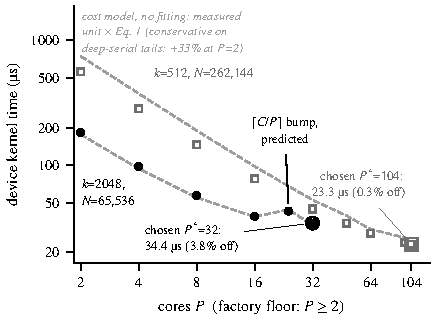
\includegraphics[width=0.76\columnwidth]{fig-e1-pscaling}
\caption{Runtime versus core count, with cost-model overlay.}
\label{fig:pscaling}
\end{figure}

\subsection{Chunk-Skip A/B}
\label{sec:eval-skip}

Fig.~\ref{fig:skipab} measures the row-parallel chunk-skip of
\S\ref{sec:system} on five cells, three arms each: baseline, skip
ungated, and skip with the compile-time $K/4$ gate. On the shapes the
small-k routing ships to this path, the gated skip wins
$\mathbf{279.14 \to 153.19}$\us{} ($-45.1\%$, $1.82\times$) at
rows${=}2$, $k{=}32$, $N{=}65{,}536$, and $279.14 \to 177.94$\us{}
($-36.3\%$) at rows${=}8$ --- the rows${=}8$ win is smaller because the
op time is the slowest of eight i.i.d.\ rows. On the three cells where
the skip law says no win exists, the gate holds the line: $+0.04\%$ and
$+0.11\%$ sit within the sub-0.1\% measurement spread, and the largest
residual, $+0.51\%$ at $k{=}512$, is the gate-off code path itself ---
loop-code growth on the in-order RISCs, not the skip test. The column-parallel guard cell
re-measures at 13.15\us{} with byte-identical kernels: the tree path is
untouched.

These measurements close the pre-build forecast's loop
(\S\ref{sec:forecast}): the no-go'd column-parallel variant was never
built; the redirected row-parallel variant landed inside the
predicted regime. One epistemic limit stands: no on-device skip-rate
telemetry was captured, so the measured quantity is end-to-end time ---
the chain runs law $\rightarrow$ simulated skip $\rightarrow$ predicted
time $\rightarrow$ measured time.

\begin{figure}[t]
\centering
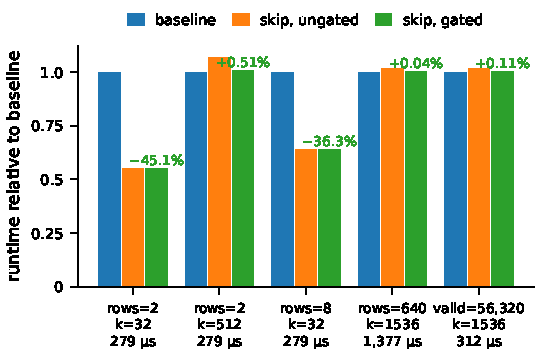
\includegraphics[width=0.76\columnwidth]{fig-e2-skip-ab}
\caption{Chunk-skip runtime relative to baseline.}
\label{fig:skipab}
\end{figure}

\subsection{Production Call-Site Scenarios}
\label{sec:eval-scenarios}

Table~\ref{tab:scenarios} replays eight production call-site shapes on
the same gated harness --- the three consumer classes of the data
contract (\S\ref{sec:bg-problem}) at their real shapes. The wins concentrate
where production is single-core today. The Qwen3 shape that opened the
paper --- the vocabulary shard padded to the one power-of-two width that
fails the $W < 65{,}535$ gate --- improves from its 9,596.3\us{}
single-core chain to 217.0\us{} routed and 193.8\us{} direct
($44$--$50\times$); split-vocab sampling on a single chip (deliberately
unpadded, $N{=}64{,}128$) behaves the same:
$8{,}923.6 \to 215.2$\us{} routed, 188.1\us{} direct.

The table carries its own no-change controls as features. The TP${=}8$
shape already rides the multi-core bitonic:
routed measures $1.00\times$ --- the honest already-fast row (the
direct op still gains $1.4\times$). The sparse-attention indexer rows
already call the op by name --- today \emph{is} the op, row-parallel
with the chunk skip live --- and forcing them through generic routing
would cost 20--25\%. The MoE gate rows are shapes the routing predicate
declines today ($W \geq 4{,}096$ floor, a measured-region choice); the
op --- $k$ rounded up to 16 and sliced, the route's own internal
mechanism --- measures 4.07\us{} and 4.04\us{} against 24.2\us{} and
77.5\us{} single-core ($5.9\times$/$19.2\times$); a route extension
still needs an A/B against the layout-envelope cost at these shapes.

One caveat is mandatory: the production sampling call sites pass
pre-allocated index tensors, sub-core grid pinning, and
\texttt{stable=True} --- each independently disqualifies routing as-is.
The routed column is the \emph{canonical} call form with
those arguments dropped --- a one-line call-site change, not a free
win --- and the end-to-end tokens/s effect of that change is
unmeasured.

\begin{table*}[t]
\centering
\caption{Production call-site scenarios with built-in controls.}
\label{tab:scenarios}
\scriptsize
\setlength{\tabcolsep}{4.5pt}
\begin{tabular}{@{}lrrrrrrrr@{}}
\toprule
call site & rows & $N$ & $k$ & today \us{} ($P$) & routed \us{} ($P$) & op \us{} ($P$) & today$\to$routed & today$\to$op \\
\midrule
Qwen3 decode sampling, TP=4 (pad) & 32 & 65,536 & 32 & 9,596.3 (1) & 217.0 (130) & 193.8 (130) & 44.2$\times$ & 49.5$\times$ \\
decode sampling, TP=8 (pad, pow-2) & 32 & 32,768 & 32 & 171.4 (65) & 171.3 (65) & 121.0 (130) & 1.00$\times$ & 1.4$\times$ \\
Llama-3.2 split-vocab sampling & 32 & 64,128 & 32 & 8,923.6 (1) & 215.2 (130) & 188.1 (130) & 41.5$\times$ & 47.4$\times$ \\
DeepSeek-V3.2 sparse-attn indexer & 160 & 65,536 & 2,048 & 712.5 (130) & 892.7 (130) & 712.5 (130) & 0.80$\times$ & 1.00$\times$ \\
DeepSeek-V4 sparse-attn indexer & 160 & 65,536 & 512 & 559.5 (130) & 691.1 (130) & 559.5 (130) & 0.81$\times$ & 1.00$\times$ \\
MiniMax MSA block selection & 1 & 8,192 & 16 & 8.4 (16) & 116.1 (65) & 8.4 (16) & 0.07$\times$ & 1.00$\times$ \\
MoE expert gate, top-4 of 128 & 32 & 128 & 4 & 24.2 (1) & --- & 4.07 (130)$^{*}$ & --- & 5.9$\times^{*}$ \\
MoE gate fallback, top-10 of 512 & 32 & 512 & 10 & 77.5 (1) & --- & 4.04 (130)$^{*}$ & --- & 19.2$\times^{*}$ \\
\bottomrule
\end{tabular}

\smallskip
\raggedright\scriptsize
All rows Tracy-measured, provenance-stamped, iteration counts recorded.
``today'' is the engine production selects now: single-core linear
(rows 1, 3, 7, 8), 65-core stock bitonic (rows 2, 6), or the op itself
(rows 4--5, chunk skip live). Op cells include the values output
(verified elementwise): $\leq$0.2\% over indices-only at sampling
shapes, ${\approx}6\%$ at the tiny gate shapes. Core counts are launched
grids ($\min(\text{rows}, 130)$ active on the row-parallel path).
$^{*}$$k$ rounds up to 16 (the op's floor) and slices; the routing
predicate declines these shapes today.
\end{table*}

\subsection{Gap to the Vendor Roofline}
\label{sec:eval-roofline}

The last two data columns of Table~\ref{tab:competition} compare the op
against the vendor's published roofline for this part, including its
$k$-dependent multipliers (0.612/0.850/1.000 for
$k{=}512$/1{,}024/2{,}048)~\cite{ttllmperf2026}. The measured gap spans
$9.7\times$--$29.9\times$ over all 24 cells and narrows to
$9.7\times$--$21.1\times$ on the $N \geq 32{,}768$ cells, shrinking
monotonically with $N$ at every $k$. The known contributors are
measured elsewhere: the comparator critical path inside each $M$-wide
leaf pass (\S\ref{sec:design-space}), the $\lceil \log_2 P \rceil$ tree
levels priced by the cost model (\S\ref{sec:system}), and the unpack
floors that tax every datum entering the SFPU
(\S\ref{sec:characterization}).
Whether the roofline is attainable at all for comparator-based kernels
--- or sits below their critical-path floor --- is a derivation we do
not print here \missing{roofline-v2 derivation artifact (G6)}; we
report the measured gap and leave feasibility open.

% Related work + methodology + conclusion -- owned by briefs/07-related.md.
% Budget: 2.0 columns (related ~0.9, methodology ~0.7, conclusion ~0.4).
% Cross-section references use the shared labels defined in each section
% stub (sec:background/design-space/system/characterization/evaluation).
% Evidence: every number below traces to paper-topk/evidence/paper/evidence.md
% (H1, H3, C3-1..C3-4, M1--M5) and RADIX_BUCKET_GPU.md SS5.2/5.3/7.4.
% PRE-SUBMISSION: read focus2025 full text; check KForge's target list for
% Tenstorrent (if present, add one sentence: kernel synthesis vs design-space
% adjudication); locate archived Blackhole microbench PDF.

\section{Related Work}
\label{sec:related}

This section carries the deltas by contribution; inline citations
appeared in context.

\paragraph{Mesh selection theory}
Krizanc and Narayanan solved rank selection on mesh-connected processor
arrays three decades ago: optimal algorithms on the abstract $n \times n$
mesh~\cite{krizanc1992optimal}, a deterministic $1.45n$-step bound against
the $2n+o(n)$ sorting bound~\cite{krizanc1993fast}, and the multi-packet
$N/p$-per-PE regime our $\lceil C/P\rceil$ leaf term
inhabits~\cite{multipacket1992}. The theory assumed unit-cost neighbor
communication and returned the $k$-th element alone: no full top-$k$ set
with values and indices, no real NoC costs, no atomics-free rendezvous,
no measurement. We therefore claim the first \emph{measured,
cost-modeled} full top-$k$ on commercial NoC-mesh silicon, with
\costmodel read as the mesh-theory bound instantiated with measured
constants (Section~\ref{sec:system}). Fagin's threshold algorithm and its
distributed descendants~\cite{fagin2003optimal,cao2004tput,michel2005klee}
merge per-node top-$k$ lists under running thresholds --- the same
tournament idea at datacenter round-trip costs.

\paragraph{GPU selection}
The GPU lineage runs from Alabi et al.~\cite{alabi2012kselection} through
WarpSelect~\cite{johnson2019billion}, Dr.~Top-$k$~\cite{gaihre2021drtopk},
the SC'23 study~\cite{zhang2023paralleltopk}, and
RadiK~\cite{li2024radik}, with database-side~\cite{shanbhag2018topk} and
row-wise~\cite{xie2024rtopk} variants; TPU-KNN~\cite{chern2022tpuknn} and
two-stage schemes~\cite{twostage2025} take the approximation escape hatch
instead. None of this lineage was ever re-costed on a machine without
atomics or scatter --- that re-costing is
Section~\ref{sec:design-space}.

\paragraph{Running-threshold pruning}
WarpSelect discards elements below a per-lane running $k$-th value before
they touch its bitonic queues~\cite{johnson2019billion} ---
element-granular, with no analytic skip law. GVR predicts the threshold
from the previous decode step and must verify and refine wrong guesses;
it reports 1.88$\times$ over TensorRT-LLM's radix select on NVIDIA
Blackwell~\cite{gvr2026}. Chunk-skip (Section~\ref{sec:system}) skips at
chunk granularity, is sound by construction --- no verification pass
exists to run --- and its distribution-free law (Eq.~\ref{eq:skiplaw})
yields a compile-time $K/4$ gate and a pre-build forecast. SpAtten's
quick-select engine~\cite{wang2021spatten} and Focus's streaming
concentrator~\cite{focus2025} are hardware threshold-engine cousins. The
rank statistics are textbook --- a running top-$k$ over a random-order
stream updates $k\ln(n/k)+O(k)$ times~\cite{knuth1998taocp3} --- but we
find no published chunked corollary, compile-time gate, or soundness
proof for skipping inside a bitonic cascade.

\paragraph{Accelerator characterization}
Published Tensix studies characterize performance --- stencils on
Grayskull~\cite{brown2024grayskull}, matmul~\cite{matmul2025tenstorrent};
FFT~\cite{brown2025fft}, stencils~\cite{stencil2026wormhole}, numerical
kernels~\cite{numkernels2026wormhole}, operator
fusion~\cite{fusion2026tensix}, and N-body~\cite{amati2025nbody} on
Wormhole. An informal Blackhole microbenchmark report
circulated in 2025, but its link is dead and no archive
exists~\cite{blackholemicrobench2025} --- itself an argument for
archival characterization. None covers datapath numerics or selection
primitives. Section~\ref{sec:characterization}'s delta over the software
float re-encodings~\cite{herf2001radix,merrill2011radix} and
IEEE~754-2019 \texttt{totalOrder}~\cite{ieee754-2019}: the Tensix
datapath imposes the total order and the bf16 canonicalization in
\emph{hardware}, not software.

\paragraph{The class-wide gap}
We find no sorting or selection publication for Cerebras WSE, Groq,
SambaNova, Occamy~\cite{occamy2025}, Manticore~\cite{zaruba2021manticore},
or Esperanto silicon; Graphcore ships \texttt{popops::TopK} with no
published algorithm or performance study~\cite{poplar_topk}. This paper
prices the ingredients any member of the dataflow-mesh class must pay ---
but fills the gap for only one member.

\section{Methodology: An Agentic Design-Space Campaign}
\label{sec:methodology}

An LLM-agent campaign with human review produced these measurements.
Prior agentic kernel work
optimizes \emph{given} kernels against benchmark
suites~\cite{ouyang2025kernelbench,sakana2025aicuda,accelopt2025,kforge2025,peak2025};
this campaign ran a design-space study with measured no-gos on
novel silicon --- we claim no first-ness for the approach, only its
record.

% ---- Optional Tab M1 (gate ledger). Cut per BUDGET.md overflow rule 3;
% re-enable if global assembly finds the column.
% \begin{table}[t]
% \centering
% \caption{Pre-registered gates and verdicts.}
% \label{tab:gates}
% \footnotesize
% \begin{tabular}{@{}p{0.16\linewidth}p{0.34\linewidth}p{0.38\linewidth}@{}}
% \toprule
% Gate & Pre-registered rule & Verdict $\rightarrow$ banked \\
% \midrule
% 1 Contract + baseline & pin semantics, build, and harness before quoting any speedup & passed $\rightarrow$ bf16 canonicalization (Sec.~\ref{sec:characterization}); the small-$k$ routing hole (Sec.~\ref{sec:evaluation}) \\
% 2 Materiali\-zation first & no complete emit path with headroom $\Rightarrow$ stop selector work & failed $\rightarrow$ materialization is the load-bearing gap (Sec.~\ref{sec:design-space}) \\
% 3 Engine shootout & report slope, fixed cost, and exact bin equality per counting arm & counting narrow (SFPU) or slow (RISC) $\rightarrow$ ingredient table (Sec.~\ref{sec:design-space}) \\
% Stop rule & build only if incumbent $\geq 2\times$ the measured-component model & fired $\rightarrow$ radix track closed; primitives banked (Sec.~\ref{sec:characterization}) \\
% \bottomrule
% \end{tabular}
% \end{table}

The campaign ran as research~$\rightarrow$~implement~$\rightarrow$~validate
gates with stop rules registered before any measurement --- a contract
gate (semantics and harness pinned first), a materialization gate (no
complete emit path with headroom $\Rightarrow$ stop selector work), and
an engine shootout; the radix track
died by its own rule (Section~\ref{sec:dspace-closure}).

The most transferable instrument was forecast-before-build
(Section~\ref{sec:forecast}): a calibrated host simulation no-go'd the
column-parallel chunk-skip variant --- never built --- and redirected
the build to the row-parallel variant that measured $-$45.1\%
(1.82$\times$) on silicon (\S\ref{sec:eval-skip}).

Agent-generated numbers earn trust only under adversarial audit: a
multi-agent audit re-verified the working notes' citations
($\approx$55 of 60 exact, none fabricated), re-adjudicated disputed
figures on fresh silicon, and caught a
faster-and-wrong kernel class with schedule-mutation controls --- the AI
CUDA Engineer's reward-hacking failure mode~\cite{sakana2025aicuda}. Correctness gates make the audit decidable:
every cell fails closed against a bit-exact golden
(\S\ref{sec:eval-method}), so wrong-but-close kernels cannot survive. The
campaign also surfaced, and reported upstream, two vendor perf-harness
bugs: a stimuli configuration never written, and a semaphore leak that
deadlocks later tests on an un-reset device.

The process also failed in ordinary ways: the a-priori Dst-layout
derivation was wrong until calibration dumps replaced it
(\S\ref{sec:char-dst}), and one working-note figure was invented
outright until the audit deleted it; both are logged in the released
notes, and neither reached a measured claim.

\section{Conclusion}
\label{sec:conclusion}

We measured exact top-$k$ across its design space on a \bh \pca and closed
a four-orders-of-magnitude gap: 631.5\,ms $\to$ 63.4\us{}
(9{,}956$\times$) at the anchor shape, 23.3\us{} on 104 cores at the
1M-context shape under the validated cost model, 1.82$\times$ more from
sound chunk-skipping in the forecast-selected row-parallel
regime. The design-space answer: on a NoC mesh without scatter, the
winning economics are parallelized comparison networks (A) plus sound
rank-statistic skipping --- the weak form of (D) --- which is
Floyd--Rivest's lesson~\cite{floydrivest1975}, not radix's.

The negative result ships with its own expiry conditions --- the counting
family (B) reopens if any one holds: (1)~a device-side compaction or
gather primitive appears, or a composed producer$+$consumer
compressed-stream benchmark proves $\geq 2\times$ headroom at $k{=}2048$,
$N \geq 262{,}144$ --- restoring true (D); (2)~$k$ outgrows the
2048-element LLK ceiling, ending the additivity of counting passes;
(3)~the consumer becomes a sampler that never materializes the top-$k$
set; (4)~$N$ grows until full-data passes (C) dominate. Future work
follows the open gaps: a Wormhole port, energy alongside
time, condition~(1)'s composed compressed-stream benchmark, and
end-to-end tokens/s once call sites drop the disqualifying arguments.


\balance
\bibliographystyle{IEEEtran}
\bibliography{refs}

\end{document}
